
\section{Motivation}

\acf{UAS} are expected to proliferate in low-altitude airspace over the coming decade. Drones with vertical takeoff and landing (VTOL) capability have been proposed to offer fast package delivery, monitor and secure assets, perform inspections, and entertain.
% The \acf{FAA} estimates over 1.25 million \acf{sUAS} were flown in 2018 \cite{federal_aviation_administration_unmanned_2019}, far exceeding the number of registered manned aircraft in the USA.  Many \ac{sUAS} are  configured for \acf{VTOL} because of requirements for minimal area for ingress and egress in cities.  
Low-altitude operation of UAS in urban areas will require flight near buildings and over people. 
% Safety must be a top priority for system designers and regulators as UAS will pose new risks to the overflown population.
A primary safety concern is ensuring a robust urgent landing capability \cite{winnefeld_unmanned_2011,degarmo_issues_2013}.  Urgent landing requires landing site selection, trajectory planning, and stable flight control to actually reach the selected site \cite{atkins_emergency_2006}. It is possible a \ac{UAS} may identify a safe site within sensor range allowing for an immediate landing.  However, when no safe site is within range the UAS must devote time and energy to exploring sites beyond sensor range or else utilize pre-processed data to identify a safe site \cite{ten_harmsel_emergency_2017,ochoa_fail-safe_2017}.  An onboard database of maps including landing sites can be incorporated into an efficient autonomous decision making framework \cite{sankararaman_towards_2017}. Offline data sources such as satellite images, airborne LiDAR point clouds, and existing map data may be used to aid map construction.
% Such a framework should incorporate risk models which account for both the intrinsic risk of the landing site as well as the path risk to reach the landing site.
% For example, Refs.  \cite{atkins_emergency_2006, meuleau_emergency_2009}  and \cite{sankararaman_towards_2017} utilize airborne flight risk models to build emergency landing plans for fixed-wing and urban flight operations, respectively. We call such a decision making framework a map-based planner.

\begin{figure}[!h]
    \centering
  \begin{subfigure}{.40\linewidth}
    \centering
    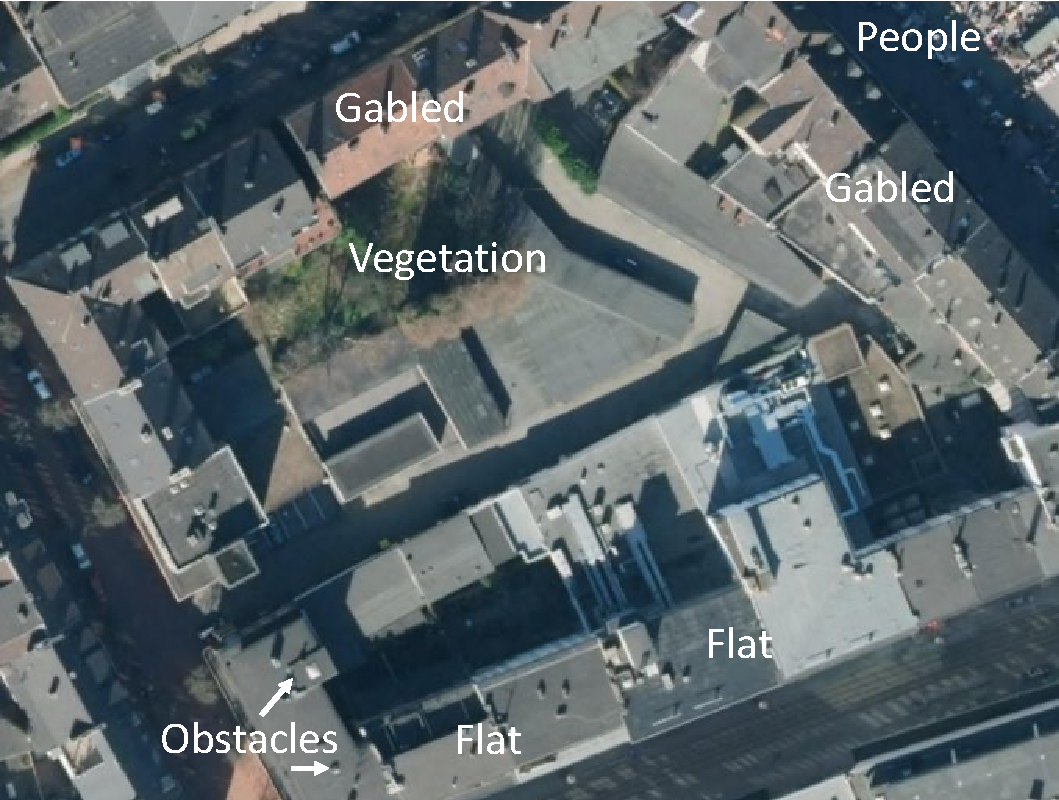
\includegraphics[page=1,clip, trim=0.0cm 0cm 0cm 0.0cm, width=0.95\linewidth]{chapter_1_intro/imgs/Motivation.pdf}
    \caption{}
    \label{fig:ch1_challenge_urban}
  \end{subfigure}
  \begin{subfigure}{.40\linewidth}
    \centering\includegraphics[page=2, width=.95\linewidth]{chapter_1_intro/imgs/Motivation.pdf}
    \caption{}
    \label{fig:ch1_roof_shape_obstacle}
  \end{subfigure}
  \caption[Motivation for rooftop landing]{Motivation for rooftop landing. (\subref{fig:ch1_challenge_urban}) Satellite image of an urban environment with multiple flat rooftops. Select roof shapes and obstacles are labeled.  (\subref{fig:ch1_roof_shape_obstacle}) A rooftop surface can be represented as a non-convex polygon with an exterior shell (green) and interior hole(s) (orange).  }\label{fig:ch1_motivation}
\end{figure}


Conventional fixed-wing emergency landing sites such as open fields and empty roadways are extremely rare in and around cities. Consider the satellite image in Figure \ref{fig:ch1_challenge_urban} which shows the typical sparsity of conventional landing zones in the city Witten, Germany. However, these images show a multitude of unoccupied flat rooftops that may provide nearby landing sites for small lightweight UAS. Obstacles such as air conditioning units, skylights, and rooftop entrances on these surfaces may be present and must be explicitly modeled and avoided during an urgent landing. Polygons can accurately and simply represent these flat surfaces as well as obstacles embedded on them per Figure \ref{fig:ch1_roof_shape_obstacle}. Archived data can be processed such that rooftop landing sites substantially augment existing conventional landing site databases.




\section{UAS Emergency Landing Background}


% How looking at usable area is a big deal
% With rooftop you now have hundreds. Need an efficient planner to choose the best one.

\ac{UAS} may experience a number of anomalies requiring emergency landing such as low battery energy, lost communication link, adverse weather, sensor or actuator failure, or operator emergency landing directives. Currently available \ac{UAS} emergency recovery capabilities are limited to simple methods such as loitering or returning to a predefined waypoint such as the launch location \cite{Stansbury2015, mejias_alvarez_forced_2009}. However, loitering or returning to a distant waypoint may present a higher level of risk to the overflown population and property compared to landing at nearby alternative sites. For this reason, emergency landing research has held a long term focus on autonomous landing site selection and trajectory generation. This dissertation defines related terms as follows. 
\begin{definition}[Prepared Landing Site]
An area designated for aircraft landing, e.g., runways, heliports, and vertiports. Surface improvements ensure suitable size, shape, and slope characteristics.  Markers maximize visibility. Protective barriers and routine inspections minimize probability of obstacles/debris.
\end{definition}
\begin{definition}[Unprepared Landing Site]
An open area with no improvements or protections, e.g., fields, roadways, and rooftops. Landing requires a visual assessment to identify or validate a suitable touchdown point.
\end{definition}
\begin{definition}[Touchdown Point]
The geographic point within a landing site area where the aircraft intends to first contact the surface.
\end{definition}
The landing site selection process is typically accomplished by utilizing on-board sensors or a database of prepared/unprepared landing sites \cite{warren_enabling_2015, ten_harmsel_emergency_2017}.  Prepared landing sites can be assumed capable of supporting a safe landing provided no other traffic is present.  Unprepared landing sites can be mapped {\em a priori} or identified in real-time.  Unprepared sites are not protected thus must be confirmed safe prior to touchdown.
\paragraph{On-board Sensors}

On-board exteroceptive sensors including camera, radar, and LiDAR can provide a wealth of information about the surrounding environment for use in emergency landing planning. However, the range and field-of-view of the sensor will limit the amount of useful data available. Vision-based systems that employ monocular cameras are widely used because they are lightweight and low cost \cite{jin_-board_2016}. Much research focuses on finding landing pads or predefined targets within images using computer vision techniques \cite{yang_autonomous_2014}. Unprepared and unstructured landing sites are found by identifying flat surfaces with sufficient size and shape characteristics within images \cite{warren_enabling_2015}. Many of these methods find unprepared landing sites from a single image or from multiple images. Single image methods utilize techniques like Canny edge detectors and assume homogeneous textures indicate planarity \cite{Wu2018, YuFeiShen2013}. \ac{SfM} algorithms may convert multiple images into points clouds to constructs height maps for planarity assessment \cite{forster_continuous_2015, desaraju_vision-based_2015}. LiDAR sensors offer a significant increase in range, precision, and accuracy but at the cost of increased expense and weight. Fully autonomous landing of helicopters utilizing only on-board LiDAR has been demonstrated \cite{scherer_autonomous_2012, theodore_flight_2006}. A fusion of sonar and LiDAR for small UAS landing site identification has also shown to be effective at finding unprepared landing sites \cite{papa_uas_2018}. However, all such methods require unprepared landing sites to be within range of on-board sensors.



\paragraph{On-board Database}

Increased data availability, low-cost storage, and accessible cloud-based infrastructure provide new opportunities for \ac{UAS} risk management. A \ac{GIS} allows free or low-cost access to a variety of geographic data including elevation maps, man-made structures, land use, and population density.  Table \ref{table:ch1_datasources} lists \ac{GIS} database sources and their use in prior research to support \ac{UAS} emergency landing. Prior work demonstrates combining and analyzing a variety of data sources to identify unprepared landing sites and accompanying maps for trajectory generation. Additionally, risk models are formulated allowing an autonomous decision framework to choose from multiple candidate landing sites.

\begin{table}[ht]
\centering
\caption{Data sources proposed for small UAS contingency management plans.}
\label{table:ch1_datasources}
% \resizebox{\columnwidth}{!}{
\begin{tabular}{@{}lll@{}}
\toprule
Information Type & Reference & Source \\ 
\midrule
\multirow[t]{3}{*}{Elevation Data}                   & \cite{bleier_risk_2015, garg_terrain-based_2015} & Shuttle Radar Topographic Mission (SRTM) \\
                                                     &  \cite{ten_harmsel_emergency_2017} & US Geological Survey, National Elevation Set \\
                                                     &  \cite{frantis_emergency_2011, yan_safe_2020, maturana_3d_2015} & Airborne LiDAR Point Clouds \\
                                                     & & \\
                                                  
\multirow[t]{3}{*}{Structures/Buildings}            & \cite{ten_harmsel_emergency_2017} & New York City Land Use Tax-lot \\
                                                    & \cite{di_donato_evaluating_2017, bleier_risk_2015}  & OpenStreetMap \\
                                                    & & \\
                                                    
\multirow[t]{3}{*}{Land Use Type}                   & \cite{ten_harmsel_emergency_2017} & US Geological Survey, National Land Cover Dataset \\
                                                    & \cite{di_donato_evaluating_2017, bleier_risk_2015} & OpenStreetMap \\
                                                    & & \\
                                                  
\multirow[t]{3}{*}{Population}                      & \cite{ten_harmsel_emergency_2017, poissant_mitigation_2020} & US Census, LandScan \\
                                                    % & \cite{poissant_mitigation_2020}   & LandScan \\
                                                    & \cite{melnyk_third-party_2014-1}  & National Human Activity Pattern Survey \\
                                                    & \cite{di_donato_evaluating_2017}  & Mobile Phone Call Detail Records \\
                                                  
\bottomrule
\end{tabular}
% }
\end{table}

\paragraph{Rooftop Landing}

All references in Table \ref{table:ch1_datasources} strictly focus on identifying and assessing risk for terrain-based landing sites such as open fields or roadways. Per. \cite{jin_-board_2016} there has been significantly less research conducted on using building rooftops for landings. Only emerging small UAS are sufficiently lightweight to land on an unprepared roof without risking structural damage or collapse. Ref. \cite{li_development_2015} proposed rooftop landing methods that rely on pre-positioned landing pads to guide landing site selection and pose estimation. However, this approach assumes a rooftop has already been established as a prepared site, whereas only a few manned helicopter vertiports have actually been established in each urban area today. Ref. \cite{desaraju_vision-based_2015}  uses a monocular camera and employs a dense motion stereo approach for 3D reconstruction while assessing planarity and slope for appropriately-sized landing sites. However, this method is limited to identifying rooftop landing sites only within the camera field of view and at low altitudes. Our work shows that there may be hundreds of viable rooftop landing sites within 200 meters of a small \ac{UAS} randomly positioned in a dense urban environment.

% building owners in cities will pay for such an expense and thus will significantly reduce the number of rooftop landing sites

% Many landing site identification and selection algorithms have been developed to process 



% Ref \cite{di_donato_evaluating_2017} uses data such as census records, Open Street Maps (OSM), and mobile phone records to quantify risk for unmanned aircraft requiring an emergency landing. Landing sites such as open fields, grasslands, and highways are identified, risk evaluated, and stored in a landing site database. The proposed planning architecture uses this on-board database to select a risk-optimal landing site within a feasible flight footprint. After a landing site is chosen, path planning is performed at a constant altitude, assessing risk to people through a fusion of census data and mobile phone activity.

% Ref \cite{ten_harmsel_emergency_2017} proposes the use of three dimensional risk grids to identify landing sites and perform path planning for an energy-constrained multicopter in urban environments. A 3D occupancy grid to represent risk is generated as a combination of terrain, population, and obstacle costs.  Terrain risk is evaluated using slope as well as terrain type, census data is used to determine population risk, and property risk is assigned equally to all buildings. A linear combination of these risks is used to generate a final 3D grid for flight planning. In this grid a landing site is a \emph{terrain} cell that has a lower cost than a configurable threshold. All landing sites are treated equally, meaning the first landing site found by the planner is the ``optimal'' choice returned.

% However none of this research addresses 


% Planners using a combination of maps and on-board sensors can capitalize on both data sources \cite{ten_harmsel_emergency_2017}. 

% Previous work all focuses on open landscapes and/or runways and considers only a single landing site in each planning epoch. 


% A meta-level framework to unify sensor and map-based planning has been proposed for general (fixed-wind) aviation \cite{atkins_emergency_2006} as well as multicopter UAS \cite{ten_harmsel_emergency_2017} as shown in Fig. \ref{fig:ch5_meta-level-planner}. This planner relies on local sensor data to land if the immediate area is safe but calls a map-based planner otherwise. Sensor and map based methods can be merged to capitalize on each other's strengths. 




% We propose map-based planning with consideration of rooftop landing sites and dual risks from landing path and site for the first time in this chapter.  Previous research in sensor-based planning, map-based planning, and multi-goal planning is summarized below.

% There are two main approaches in generating landing sites for use in map-based UAS emergency landing: one producing a specific landing site database and the other generating a risk grid from which landing sites can be selected.


% Ref. \cite{primatesta_ground_2020} proposes generation of a 2D risk map that quantifies  risk to population on the ground. The map is created taking into account an aircraft's model parameters and the local environment conditions while considering their uncertainties. The risk map is defined for a specific altitude and is the combination of several risk layers including population density, obstacles, sheltering, and no fly zones.

% \section{Data Background}

\section{Geographic Information System Background}

A \acf{GIS} is a framework to acquire, label, and update geographic data that model economic, environmental, and social properties \cite{antenucci_geographic_1991}. Each GIS data record is marked by a geographic location in an Earth-referenced coordinate frame.  Earth-referenced coordinate systems allow heterogeneous data to be aligned in  multi-layer maps. This dissertation utilizes three main \ac{GIS} data types: raster, vector, and point cloud data.  Publicly available point cloud data are becoming increasingly available worldwide from both regional and federal governments. Figure \ref{fig:ch1_gis_types} shows \ac{GIS} data examples.

% A brief overview of common \ac{GIS} coordinate systems is provided below.


\begin{figure}[!htb]
  \centering
  \begin{subfigure}[t]{.30\linewidth}
    \centering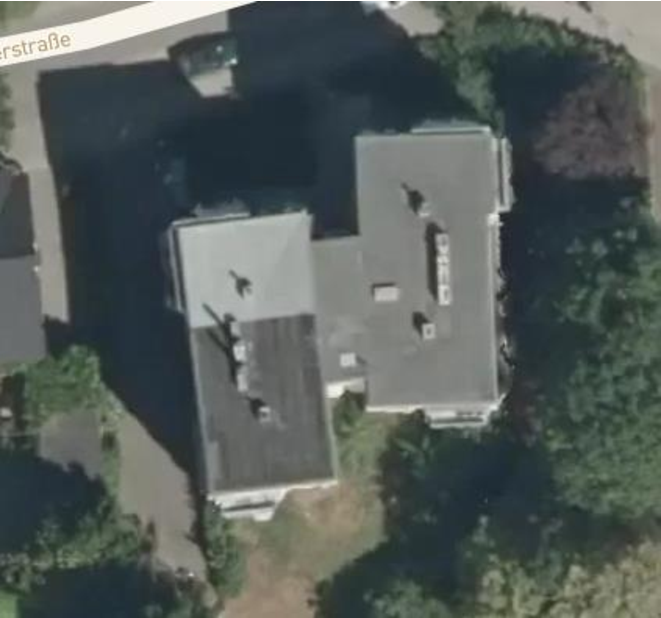
\includegraphics[page=1,clip,trim=0cm 0cm 0cm 0cm,width=.99\linewidth]{chapter_1_intro/imgs/gis_types.pdf}
    \caption{\label{fig:ch1_gis_type_a}Raster, Satellite Image}
  \end{subfigure}
  \begin{subfigure}[t]{.30\linewidth}
    \centering\includegraphics[page=2,clip,trim=0cm 0cm 0cm 0cm,width=.99\linewidth]{chapter_1_intro/imgs/gis_types.pdf}
    \caption{\label{fig:ch1_gis_type_b}Vector, Building Outline}
  \end{subfigure}
  \begin{subfigure}[t]{.30\linewidth}
    \centering\includegraphics[page=3,clip,trim=0cm 0cm 0cm 0cm,width=.99\linewidth]{chapter_1_intro/imgs/gis_types.pdf}
    \caption{\label{fig:ch1_gis_type_c}Airborne LiDAR Point Cloud}
  \end{subfigure}
  \caption[Common data types used in GIS]{Common data types used in \ac{GIS}}\label{fig:ch1_gis_types}
\end{figure}

\paragraph{Reference Coordinate Systems}
% \subsection{Coordinate Systems}

%The most widely used \acf{GCS} is WGS84, which includes the definition of the coordinate system's fundamental and derived constants, the ellipsoidal (normal) Earth Gravitational Model (EGM), and a description of the associated World Magnetic Model (WMM) \cite{wgs84}. WGS84 is measured in degrees of longitude (x-coordinates) and latitude (y-coordinates) where positive values correspond to north of the equator and east of the prime meridian, respectively. However, this spherical coordinate system is unsuitable for use in metric distance and area calculations. Therefore \emph{projected} coordinate systems are used that map the earth's spherical surface onto a two-dimensional Cartesian coordinate plane. These are called map projections.

The most widely used \acf{GCS} is WGS84 \cite{wgs84} measured in degrees of latitude  and longitude where positive values correspond to North of the Equator and East of the Prime Meridian, respectively. This spherical coordinate system is unsuitable for use in metric distance and area calculations needed for landing site selection so projected coordinate systems map the spherical surface to a two-dimensional Cartesian  planes called map projections from which distortions can be removed \cite{GIS_demystified}.
%These map projection will have distortion in the fundamental spatial properties of distance, area, shape, or direction. However map projections have been devised to minimize or completely remove distortions for certain spatial properties to suit particular purposes \cite{GIS_demystified}. 
This dissertation utilizes the Universal Transverse Mercator (UTM) system unless otherwise noted. 
% There exists many map projection which are standardized and used throughout the world globally, nationally, and regionally. An example global map projection is the Universal Transverse Mercator (UTM) system. This dissertation will utilize the UTM system unless otherwise noted.
Data from disparate coordinate systems may be overlaid and aligned by transforming coordinates from one coordinate reference system to another. These transformation are done by specialized software, such as PROJ4 \cite{proj_contributors_proj_2018}.

% Data is georeferenced if its internal coordinate system is defined using a \ac{GCS} or a map projection. 

\paragraph{Raster Data}
% \subsection{Raster Data}

A raster is composed of a matrix of cells organized into rows and columns, where each cell represents information. Common rasters include images, digital terrain elevation models, and rasterized population density maps. 
Imagery can be captured by satellite or aircraft.  
%Figure \ref{fig:ch1_gis_type_a} shows an example high resolution satellite image. 
Satellite data offer global coverage with the highest resolution currently offered at 30 cm/pixel \cite{2041-210X.12973}.  Aerial imagery has resolutions as high as 2.5 cm/pixel \cite{SHAO2021126954, 2041-210X.12973}. 
%There are two coordinate systems within a raster: the (u,v) pixel position of each cell and the corresponding (x,y) map projection position. An affine matrix is used to convert between the two coordinate systems such that every pixel corresponds to a precise location on the surface of the earth.
% An affine matrix $A$ is used to convert between the two coordinate systems such that every pixel in the raster has a known world position:

% \begin{align}
%     A = \begin{bmatrix} \label{eq:affine_matrix}
%         x_{res} & 0 & x_{min} \\
%         0 &  -y_{res} & {y_{max}}
%         \end{bmatrix} \quad
%     \begin{bmatrix} u \\ v \end{bmatrix} = A \cdot \begin{bmatrix} x \\ y \end{bmatrix}
% \end{align}

% where $x_{res}$ and $y_{res}$ denote the metric resolution of each pixel, and $x_{min}$/$y_{max}$ are the minimal/maximal geographic bounds of the image in the x and y axes, respectively. The affine matrix allows pixel correspondence to a precise location on the surface of the earth. 

% This dissertation uses satellite images and terrain elevation models.

%\paragraph{Vector Data}
% \subsection{Vector Data}

%Vector data provides a more precise representation of the location and shape of world features in comparison to raster data \cite{GIS_demystified}. Common vector features include streets, park/field outlines, and building footprints as seen in Google Maps or \ac{OSM}. Vector features are constructed as ordered pairs of (x,y) vertices which reside on a map projection plane.  A vector feature is represented by one of four types of geometric shapes: point, polyline, linear ring, or polygon. This dissertation follows the Open Geospatial Consortium (OGC) standard \cite{herring_opengis_2006-1} for defining these geometric types which are summarized as follows. A point represents a single (x,y) position in coordinate space. A polyline is an ordered list of points where each consecutive pair of points defines a line segment. A linear ring is a polyline that is both closed and simple. This mandates a linear ring to have non-intersecting line segments that join to form a closed path. A valid polygon must have a single exterior linear ring representing the hull of the polygon and a set of linear rings (possibly empty) representing holes inside the polygon. Figure \ref{fig:ch1_gis_type_b} shows a polygon of a building footprint.

% Additionally no two rings in the boundary may cross and rings may only intersect at a singular point.

% This dissertation focuses on the creation of polygons.
\paragraph{Point Cloud Data}
% \subsection{3D Point Cloud Data}
A point cloud is a collection of 3D points defined in a Cartesian reference frame. %These points represent the (x,y,z) coordinates of an underlying sampled surface. 
Point clouds in \ac{GIS} are often generated with a top-down vantage point from aircraft outfitted with \ac{LiDAR}, \ac{GPS}, and an \ac{INS}.  \ac{LiDAR} scans are stitched together in an airborne \ac{LiDAR} point cloud. 
%Publicly available point cloud data are becoming increasingly available worldwide from both regional and federal governments. Figure \ref{fig:ch1_gis_type_c} shows a section of a LiDAR point cloud.


\section{Problem Statement}

This dissertation addresses the following challenges:

\begin{enumerate}[noitemsep]
    \itemsep0em 
    \item Where can a small UAS safely land in a city during an urgent or emergency landing situation?
    \item How can maps be constructed and risk evaluated for landing site selection and path planning?
    \item How can a small UAS verify a landing zone is safe in real-time on approach to that site?
\end{enumerate}

Previous research has proposed the use of public \ac{GIS} datasets such as satellite images, airborne LiDAR point clouds, digital elevation maps, census data, and building outlines for terrain-based landing site identification, risk assessment, and path planning \cite{meuleau_emergency_2009, di_donato_evaluating_2017, patterson_timely_2014, bleier_risk_2015}.  However increased use of \acf{sUAS} in urban cities motivates this work to additionally consider building rooftops as landing sites. To our knowledge this dissertation is the first work to explicitly use GIS data to automatically identify flat rooftop buildings, isolate flat surfaces, and find risk-minimum touchdown points that maximize distance to obstacles. 

% These conventional landing sites are often risk evaluated by terrain type and size \cite{di_donato_evaluating_2017}. 
\section{Research Approach and Thesis Outline}

% Map data is widely available in vector form, such as polygons, which describes features such as fields, parks, and building outlines \cite{openstreetmap_contributors_planet_2017}.  Such polygons can be efficiently stored and indexed such that spatial queries may efficiently computed in an embedded database \cite{furieri_spatialite_2017}. 

This dissertation proposes to process existing \ac{GIS} data to extract safe landing sites and risk evaluate for landing site selection. To accomplish this computational geometry algorithms have been developed to enable efficient extraction of flat surfaces as non-convex polygons. The overall structure of this dissertation is shown in Figure \ref{fig:ch1_thesis_overview} and can be summarized as accomplishing the following seven tasks:
% This dissertation assumes these urgent landing scenarios are without loss-of-control, for example: low battery energy, lost communication link, adverse weather, non-essential sensor or actuator failure, operator emergency landing directive, and non-cooperative aircraft nearby.

\begin{enumerate}[noitemsep]
    \item Efficiently extract non-convex polygons with interior holes from 2D point sets. (Ch. 2)
    \item Extend polygon extraction methods from 2D point sets to 3D data where polygons represent flat surfaces and interior holes represent obstacles embedded on the surface. (Ch. 3)
    \item Classify rooftop shape in a city (e.g., flat) with high confidence in model prediction. (Ch. 4)
    \item Assimilate publicly available GIS data such as satellite images, airborne LiDAR point clouds, and building outlines into an urgent landing site database with associated risk metrics as well as occupancy maps for path planning. (Ch. 5)
    \item Create a multi-goal planner to efficiently search candidate sites and account for landing site risk as well as flight path risk to that site. The planner identifies a landing site/path pair to minimize combined \emph{total} risk as well as computation time for this search. (Ch. 5)
    \item Create a real-time touchdown point selection algorithm to verify a landing zone on approach. Construct a high fidelity simulated city for testing. (Ch. 6)
    \item Perform flight experiments to verify the planned touchdown location is safe in real-time using on-board \ac{LiDAR}. (Ch. 7)
\end{enumerate}

Our research approach begins with developing methods for extracting non-convex polygons from 2D \& 3D data in Chapters \ref{ch:polylidar} and \ref{ch:polylidar3d}, respectively. Though the chapters present methods and examples which are general to many domains, this thesis will highlight their use for rooftop surface extraction. Chapter \ref{ch:roofshape} presents our methods of labelling rooftop shapes with a machine learning framework by utilizing satellite image and airborne LiDAR point clouds.  Chapter \ref{ch:maplanding} integrates polygon extraction and roof shape prediction in order to create an emergency landing site database that uniquely includes rooftops. We propose several risk metrics that allow a multi-goal planner to choose the risk-minimal landing site and path/pair. Chapter \ref{ch:landingsim} proposes methods to validate a landing site on approach by using on-board LiDAR and camera sensors. We extend Polylidar3D to integrate with semantic segmentation and show improved robustness from individual sensor failure. Finally, Chapter \ref{ch:experiments} experimentally evaluates the use of Polylidar3D for real-time touchdown point selection with on-board LiDAR.

% The final risk-optimal landing site/path pair is sent to a navigation controller.
\begin{figure}[t]
    \centering
    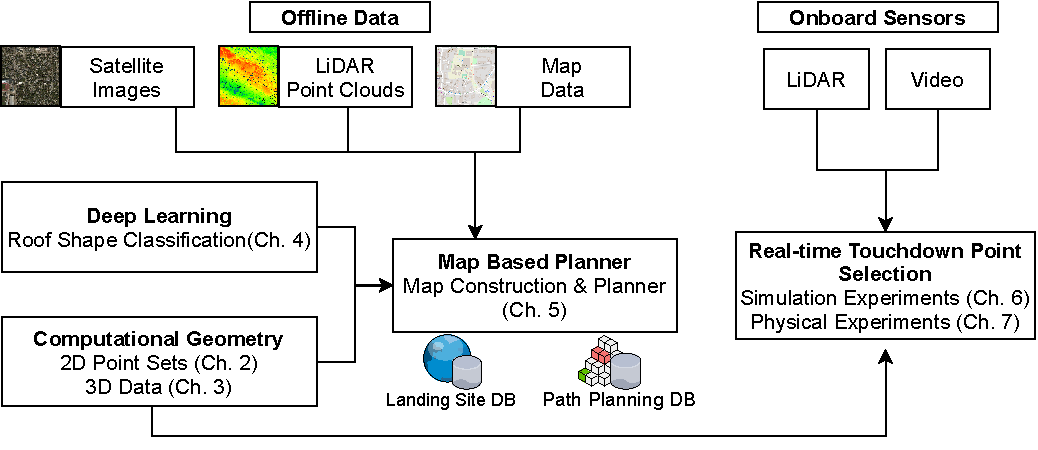
\includegraphics[width=0.80\linewidth]{chapter_1_intro/imgs/Challenge_Overview-thesis_overview.pdf}
    \caption[Overview of dissertation topics and structure]{Overview of dissertation topics and structure.}
    \label{fig:ch1_thesis_overview}
\end{figure}


\section{Contributions and Innovations}
% \vspace{1.5cm}
Specific contributions of this dissertation include: % things that have taken time / effort

\begin{itemize}[noitemsep]
  \item A faster open source library for non-convex (multi)polygon extraction from 2D point sets. An open source benchmark comparison of leading non-convex polygon extraction techniques in terms of accuracy and speed is provided. %\cite{Castagno_Github_Polylidar}.
%   \item An open source benchmark comparison of leading concave polygon extraction techniques from 2D point sets in terms of accuracy and speed.
  \item An efficient and versatile open source framework, Polylidar3D,  for non-convex (multi)polygon extraction from 3D data representing flat surfaces. Polylidar3D can handle unorganized and organized 3D point clouds as well as triangular meshes. Computation time is minimized with CPU multi-threading and GPU acceleration. %\cite{Castagno_Github_Polylidar}
  \item Multiple open source and reproducible experiments showing qualitative and quantitative benchmark results of Polylidar3D applied to sensors including LiDAR and RGBD cameras.
  \item A fast open source dominant plane normal estimation library, FastGA,  using a novel Gaussian Accumulator with efficient search.
  \item A deep learning framework for predicting roof shapes from a fusion of satellite image, airborne LiDAR point cloud, and existing building outline data. Over 4,500 buildings rooftops spanning three cities were manually classified  for training, validation, and testing.
  \item A multi-goal planner that guarantees a risk-optimal solution is found rapidly by avoiding exploration of high-risk options. Plans are optimized over a combination of landing site and path risk metrics.
  \item Experimental UAS results of real-time landing site validation or identification/selection with Polylidar3D.
\end{itemize}
 
Specific innovations of this dissertation are: % things that have taken time / effort

\begin{itemize}[noitemsep]
      \item A novel computationally-efficient algorithm to extract non-convex polygons from 2D point sets while accounting for holes. The proposed method utilizes half-edge boundary following with edge-case detection instead of alternatives such as the expensive union of triangles.
      \item The first parallelized non-convex polygon extraction framework working with several forms of 3D data. Polygons represent dominant planar surfaces with interior holes representing the shape of obstacles embedded on their surface. Polylidar3D's speed and data input versatility allow its use for many applications.
    %   Triangle primitives are grouped according to dominant plane normals for which region growing occurs in parallel. Polygon extraction of segmented planar regions are spawned as dynamic tasks in a thread-pool. 
      \item The first large-scale multi-city analysis for predicting roof shapes. The provided annotated dataset contains diverse examples from small to large metropolitan city centers. 
      \item The first rigorous method to incorporate flat rooftops as candidate landing sites for urgent landing of small UAS in cities.  Optimal touchdown sites on rooftop surface are determined using geometric methods with risk evaluated according to size and proximity to alternative touchdown sites.
\end{itemize}


\section{Products}

Publications, software, and datasets connected to this dissertation are:
\vspace{0.2cm}

\textbf{Conference}
\vspace{0.20cm}
\begin{itemize}[noitemsep]
    \item J. Castagno, C. Ochoa, and E. Atkins, ``Comprehensive Risk-based Planning for Small Unmanned Aircraft System Rooftop Landing,” in 2018 \emph{International Conference on Unmanned Aircraft Systems} (ICUAS), Jun. 2018, pp. 1031–1040, doi: 10.1109/ICUAS.2018.8453483.
    \item K. McDonough, J. Castagno, and J. Player, ``RANGR: Risk Aware Navigation and Gudiance Resilience,” presented at the \emph{AUVSI Xponential}, Denver, CO, USA, May 2018.
	\item J. Castagno and E. M. Atkins, ``Automatic Classification of Roof Shapes for Multicopter Emergency Landing Site Selection,” in 2018 \emph{Aviation Technology, Integration, and Operations Conference, American Institute of Aeronautics and Astronautics}, 2018.
\end{itemize}

\vspace{0.25cm}

\textbf{Journal}

\vspace{0.20cm}
\begin{itemize}[noitemsep]
    \item J. Castagno, Y. Yao, E. Atkins, ``Autonomous Rooftop Touchdown Point Selection". \emph{Journal of Intelligent Robot Systems}. Submitted, Under Review. 
    \item J. Castagno, M. Romano, P. Kuevor, and E. Atkins, ``Multi-UAV Wildire Boundary Estimation using a Semantic Segmentation Neural Network,” \emph{Journal of Aerospace Information Systems}, vol. 18, no. 5, pp. 231–249, 2021, doi: 10.2514/1.I010912.
    \item J. Castagno and E. Atkins, ``Map-Based Planning for Small Unmanned Aircraft Rooftop Landing," in \emph{Handbook on Reinforcement Learning and Control}, Springer, 2021. doi:10.1007/978-3-030-60990-0.
    \item J. Castagno and E. Atkins, “Polylidar3D - Fast Polygon Extraction from 3D Data," \emph{Sensors}, vol. 20, no. 17, Art. no. 17, Jan. 2020, doi: 10.3390/s20174819.
    \item J. Castagno and E. Atkins, “Polylidar - Polygons From Triangular Meshes," \emph{IEEE Robotics and Automation Letters}, vol. 5, no. 3, pp. 4634–4641, Jul. 2020, doi: 10.1109/LRA.2020.3002212.
    \item J. Castagno and E. Atkins, “Roof Shape Classification from LiDAR and Satellite Image Data Fusion Using Supervised Learning," \emph{Sensors}, vol. 18, no. 11, Art. no. 11, Nov. 2018, doi: 10.3390/s18113960.
\end{itemize}

\textbf{Open Source C++ libraries (with Python bindings)}

\begin{itemize}[noitemsep]
    \item J. Castagno, ``Polylidar3D,''   [Online]  Available: \url{https://github.com/JeremyBYU/polylidar}, 2020.
    \item J. Castagno, ``Fast Gaussian Accumulator,''   [Online]  Available: \url{https://github.com/JeremyBYU/FastGaussianAccumulator}, 2020.
    \item J. Castagno, ``Organized Point Filters,''   [Online]  Available: \url{https://github.com/JeremyBYU/OrganizedPointFilters}, 2020.
\end{itemize}

\textbf{Open Data Sets}

\begin{itemize}[noitemsep]
    \item J. Castagno, ``Annotated Roof Shape Dataset,''   [Online]  Available: \url{https://www.mdpi.com/1424-8220/18/11/3960/s1}, 2018.
    \item J. Castagno, ``Annotated Roof Asset Dataset,'' [Online] Available: \url{https://github.com/JeremyBYU/UnrealRooftopLanding/blob/master/assets/data/manhattan/buildings.csv}, 2021.
\end{itemize}
